	\documentclass[twoside]{article}
\usepackage{../../estilo-ejercicios}
\renewcommand{\baselinestretch}{1,3}
%--------------------------------------------------------
\begin{document}

\title{Ejercicios de Topología Algebraica}
\author{Javier Aguilar Martín}
\maketitle

\begin{ejercicio}{2.1.9}\
Calcular los grupos de homología del $\Delta$-complejo $X$ obtenido de $\Delta^n$ identificando todas las caras de la misma dimensión. Esto es, $X$ tiene un solo $k$-símplice para cada $k\leq n$. 

 

\end{ejercicio}
\begin{solucion}\
Es claro que $C_i(X)$ tiene una sola célula $e_i$ para cada $0\leq i\leq n$, por lo que el complejo de cadenas es simplemente
\[
0\to \Z\xrightarrow{d_n}\Z\xrightarrow{d_{n-1}}\cdots \xrightarrow{d_2}\Z\xrightarrow{d_1}\Z\to 0
\]
Como $X$ es conexo, $H_0(X)=\Z$ y esto significa que $d_1=0$. Veamos qué ocurre para $i>0$. Sea $e^i$ la célula que genera $C_i(X)$. Como $e^1\cong\Delta^i$, en $S^{i-1}=\partial e^i$ podemos encontrar abiertos disjuntos homeomorfos a las caras de dimensión $i-1$ de $\Delta^i$, que se pegan a $e^i$ con la orientación inducida por el símplice. Entonces, la aplicación $S^{i-1}\to X^{i-1}/X^{i-2}=S^{i-1}$ envía cada abierto de los descritos anteriormente a toda la esfera salvo un punto $y\in S^{i-1}$. La preimagen de todo punto $x\neq y$ consiste en un conjunto finito formado por $\binom{i+1}{i}=i$ puntos (el número de caras de dimensión $i-1$ de $\Delta^i$). Además, la orientación que induce el símplice es alternante, por lo que los grados locales alternan de signo y el grado total es $\sum_{j=0}^i(-1)^j$. Esto implica que $d_i=0$ si $i$ es impar (en particular para $d_1$, tal como habíamos calculado) y $d_1$ es isomorfismo para $i$ par. En homología esto se traduce en que $H_i(X)=0$ para todo $i\neq 1,n$, siendo $H_n(X)=\Z$ si $n$ es impar y $H_n(X)=0$ si $n$ es par. En resumen:
\[
H_i(X)=\begin{cases}
0 & i\neq 0,n\lor i=n \text{ par}\\
\Z & c.c.
\end{cases}
\]
\end{solucion}

\newpage

\begin{ejercicio}{2.1.14}
Determinar si existe una sucesión exacta corta $$0\to\Z_4\to \Z_8\oplus\Z_2\to \Z_4\to 0.$$ Más generalmente, determinar qué grupos abelianos $A$ forman una sucesión exacta corta $0\to\Z_{p^m}\to A\to\Z_{p^n}\to 0$ con $p$ primo. ¿Y en el caso de las sucesiones exactas cortas $0\to\Z\to A\to\Z_n\to 0$?
\end{ejercicio}
\begin{solucion}
Llamos respectivamente $i$ y $j$ a las aplicaciones de la hipotética sucesión exacta corta. Por ser $i$ inyectiva, $\Ima{i}\cong\Z_4$, por lo que del primer teorema de isomorfía y la exactitud obtendríamos que $\Z_8\oplus\Z_2/\Z_4\cong\Z_4$. Esto no contradice el teorema de Lagrange, ya que las cardinalidades coinciden, y de hecho, en caso de que exista un subgrupo isomorfo a $\Z_4$ de modo que el cociente sea también isomorfo a $\Z_4$, esto nos da una manera de definir $j$. Identificamos los elementos del cociente $\Z_8\oplus\Z_2/\Z_4$ con las clases de equivalencia $\{\overline{0}, \overline{1},\overline{2},\overline{3}\}$. Para todo $x\in\overline{n}$, definimos $j(x)=n\in\Z_4$. Esta aplicación es un homomorfismo de grupos porque se conserva la estructura de grupo del cociente, es claramente sobreyectiva y su núcleo son los elementos de la clase $\overline{0}$, que son justamente los elementos del subgrupo isomorfo a $\Z_4$, y por tanto coinciden con $\Ima{i}$. Así pues, consideramos el subgrupo de $\Z_8\oplus\Z_2$ generado por $(2,1)$. El grupo $\Z_8\oplus\Z_2/\gene{(2,1)}$ tiene la presentación como grupo abeliano $\gene{a,b\mid 8a=0,2b=0, 2a+b=0}$, de donde obtenemos que $4a=0$ multiplicando la tercera ecuación por 2, y  $2a=b$ entre las dos últimas, de donde deducimos que efectivamente este grupo es isomorfo a $\Z_4$ (también se podría hacer calculando la forma normal de Smith de la matriz de coeficientes). Así que basta definir $i(1)=(2,1)$ y $j$ tal como se ha explicado anteriormente.

En el caso más general, $0\to \Z_{p^m}\to A\to \Z_{p^n}\to 0$, como $A$ tiene un subgrupo cíclico $B\cong\Z_{p^m}$ y un cociente cíclico $A/B\cong\Z_{p^n}$, $A\cong\Z_r\oplus\Z_s$ para ciertos enteros $r$ y $s$, pues podemos tomar como generadores un generador de $B$ y un representante de un generador de $A/B$. Por el teorema de clasificación de grupos abelianos, se puede tomar $r|s$. Por el teorema de Lagrange, $p^mp^n=|B||A/B|=|A|= rs$. Esto nos da $r=p^i$, $s=p^{m+n-i}$ con $0\leq i\leq \min\{m,n\}$. Esto nos da una condición necesaria para $A$, veamos que es suficiente. Sean $r=p^i$ y $s=p^{m+n-i}$, con $0\leq i\leq\min\{m,n\}$. Como $i\leq m$, hay un homomorfismo sobreyectivo $\alpha:\Z_{p^m}\to \Z_{p^i}$. Por otro lado, 
\[
m+n-i\geq m+n-\min\{m,n\}=\max\{m,n\}+\min\{m,n\}-\min\{m,n\}=\min\{m,n\}\geq m
\] 
luego existe un homomorfismo inyectivo $\beta:\Z_{p^m}\to\Z_{p^{m+n-i}}$. Como $\beta$ es inyectivo, también lo es $(\alpha,\beta):\Z_{p^m}\to \Z_{p^i}\oplus\Z_{p^{m+n-i}}$. El conúcleo de esta aplicación tiene orden $p^n$ por el teorema de Lagrange, luego bastaría probar que es cíclico para comprobar que encaja en la sucesión exacta corta. Para ello, basta definir $\alpha(1)=(1,0)$ y $\beta(1)=(0, p^{m-i})$, que fácilmente se ve que verifican las condiciones de sobreyectividad e inyectividad. Ahora, el conúcleo de $(\alpha,\beta)$ tendría como presentación abeliana $$\gene{a,b\mid ap^i=0, bp^{m+n-i}=0, \alpha(1)=a=0, \beta(1)=b^{m-i}=0},$$ de donde se obtiene que es cíclico con al simplificarla eliminado $a$.


  

Por último, consideremos la sucesión exacta corta $0\to\Z\to A\to \Z_n\to 0$. Veamos que $A=\Z\oplus\Z_d$ con $d|n$ encaja en ella. Definimos $\psi:\Z\oplus\Z_d\to\Z_n$ como $\psi(x,y)=x+cy$, donde $n=cd$, que es claramente sobreyectiva. Es claro que $\ker\psi=\gene{(c,-1)}\cong\Z$, luego si definimos $\phi:\Z\to \Z\oplus\Z_d$ mediante $\phi(1)=(c,-1)$, que es inyectiva, obtenemos la exactitud. Veamos que de hecho este es el único grupo salvo isomorfismo que podemos colocar en el lugar de $A$.
    
    
Supongamos ahora que $A$ encaja en la sucesión exacta corta. Considermos entonces el siguiente morfismo de sucesiones exactas cortas
\[
\begin{tikzcd}
0\arrow[r] & \Z\arrow[r]\arrow[d, equals] &\Z\times\Z\arrow[r]\arrow[d] & \Z\arrow[r]\arrow[d] & 0\\
0\arrow[r] &  \Z\arrow[r] & A \arrow[r] & \Z_n\arrow[r] & 0
\end{tikzcd}
\]
donde $\Z\times\Z\to A$ es cualquier homomorfismo de grupos, que sabemos que existe porque $A$ es un $\Z$-módulo, y además podemos tomarlo de modo que los cuadrados conmuten: 
\begin{itemize}
\item para que el cuadrado izquierdo conmute, primero definimos $\Z\to\Z\times\Z$ como $1\mapsto (1,0)$, y después $(1,0)$ se envía a la imagen del 1 mediante $\Z\to A$.
\item para que conmute el cuadrado derecho, en primer lugar definimos $\Z\times\Z\to\Z$ como $(1,0)\mapsto 0$ y $(0,1)\mapsto 1$, de modo que $(a,b)\mapsto b\mod n\in\Z_n$. Como $A\to\Z_n$ es sobreyectiva, envíamos $(0,1)$ a la preimagen de $1\in\Z_n$.  
\end{itemize}
 El Snake Lemma nos da el diagrama conmutativo siguiente, donde denotamos $\Z\times\Z\xrightarrow{\phi} A$
\[
\begin{tikzcd}
            & 0\arrow[d] & 0\arrow[d]                  & 0\arrow[d] &\\
 0\arrow[r] & 0\arrow[r]\arrow[d] & \ker\phi\arrow[d] \arrow[r, "\cong"] & n\Z\cong\Z\arrow[r]\arrow[d] & 0\\
 0\arrow[r] & \Z\arrow[r]\arrow[d, equals] & \Z\oplus\Z \arrow[r]\arrow[d] & \Z \arrow[r]\arrow[d] & 0\\
 0\arrow[r] & \Z\arrow[r]\arrow[d] & A\arrow[r]\arrow[d] & \Z_n\arrow[r]\arrow[d] & 0\\
            &       0     &        0   &   0
\end{tikzcd}
\]
En este diagrama, los 0 que no nos da directamente el Snake Lemma surgen de completar a partir del isomorfismo $\ker\phi\cong\Z$ salvo $A\to 0$, que es consecuencia de la demostración del lema de los cinco al ser $\Z\to\Z$ isomorfismo y $\Z\to\Z_n$ sobreyectiva. La columna central es una sucesión exacta corta isomorfa a la siguiente
\[
0\to \Z\xrightarrow{(n,r)}\Z\oplus\Z\to A\to 0
\]
para algún $r$ entero. La matriz $\binom{n}{r}$ se puede reducir a $\binom{d}{0}$, donde $d=\gcd(n,r)$, lo que, usando la exactitud junto con el primer teorema de isomorfía, nos da $A\cong \Z\oplus\Z_d$.
\end{solucion}

\newpage

\begin{ejercicio}{2.2.3}
Sea $f:S^n\to S^n$ una aplicación de grado cero. Probar que existen puntos $x,y\in S^n$ con $f(x)=x$ y $f(y)=-y$. Usar esto para probar que si $F$ es un campo vectorial continuo en la bola unidad $D^n$ en $\R^n$ tal que $F(x)\neq 0$ para todo $x$, entonces existe un punto en $\partial D^n$ donde $F$ apunta radialmente hacia fuera y otro punto en $\partial D^n$ donde $F$ apunta radialmente hacia dentro.
\end{ejercicio}
\begin{solucion}
\end{solucion}

\newpage

\begin{ejercicio}{2.2.10}
Sea $X$ el espacio cociente de $S^2$ bajo las identificaciónes $x\sim-x$ para $x$ en el ecuador $S^1$. Calcular los grupos homología $H_i(X)$. Hacer lo mismo para $S^3$ con puntos antipodales del ecuador $S^2\subset S^3$ identificados. 
\end{ejercicio}
\begin{solucion}
\end{solucion}

\newpage


\begin{ejercicio}{de las naranjas}
Para el espacio $X$ de la imagen (donde las esferas se consideran huecas), calcular la homología local de todos sus puntos, hallar la mayor cantidad posible de subespacios $A\subseteq X$ tales que cualquier homeomorfismo $f:A\to X$ satisfaga $f(A)\subseteq A$, y estudiar si es posible asegurar que alguna potencia $f^n$ tenga puntos fijos, y en su caso cuántos. 

\begin{figure}[h!]
\centering
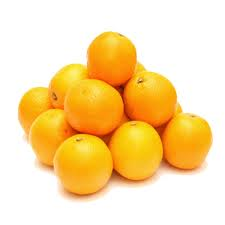
\includegraphics[scale=0.5]{naranjas}
\end{figure}
\end{ejercicio}

\end{document}
